\section{Exercise 4}
\subsection{ex4-a}
\begin{table}[!htbp]
\begin{tabular}{|l||l|l|l|l|l|l|l|l|}
\hline
Training iterations $\rightarrow$  & 1   & 2 & 3 & 4 & 5 & 6 & 10 & 50 \\ \hline
Validation accuracy  & 63\% & 60\% & 55\% & 55\% & 56\% & 56\% & 56\% & 56\% \\ 
Testing accuracy    & 57\% & 57\% & 48\% & 54\% & 54\% & 54\% & 54\% & 54\% \\ \hline
\end{tabular}
\end{table}
The perceptron goes through the examples same way as they are ordered in trainingData. 
The element that is on position 0 in trainingData will be processed first.
Whether or not the perceptron is better than Naive Bayes depends heavily on the options 
one might change when training on the data. As follows from the data given in section 2.1 
Naive Bayes gets a 69\% score for validation and a 55\% score for testing with a K of 2. \\
If you compare this to the score of the perceptron with 5 iterations then the Naive Bayes 
classifier is obviously better because both the validation and testing score is higher.
However, when you compare it with the perceptron with 1 or 2 training iterations, the perceptron
scores are better. \\
The Naive Bayes validation accuracy might be higher but the testing accuracy
is the important score because this will give the best indication for future scores. 
The testing accuracy is higher with 57\% versus 55\%.
But once you use autotune to get a better score for Naive Bayes, it is significantly better
than the best score of the perceptron with a validation accuracy of 74\% and a testing accuracy 
of 65\% for a K of 0.1. So in most cases the Naive Bayes classifier is better than the perceptron.

\subsection{ex4-b}
Based on the scores collected in part 4.1 it is safe to stop training after 5 iterations. 
This is because the scores you get when training even more are not better than after 5 iterations, 
in fact, they are exactly the same. However, when faced with a different training set it is 
possible that the perceptron's score keep improving after 5 iterations.

\subsection{ex4-c}
\begin{figure}[H]
\caption{}
\centering
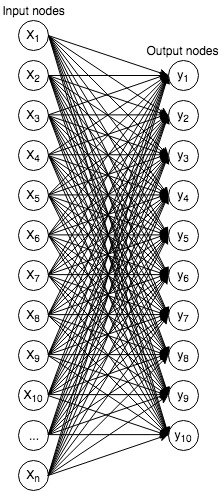
\includegraphics[width=6cm]{4c2}
\end{figure}
The activation function for the perceptron is $y_j$ = $\sum_{i=1}^{n} X_i * w_i^j$. Here every 
connection has a weight $w_i^j$ where i indicates the input node and j indicates the output node.
